\documentclass[conference]{IEEEtran}
\usepackage{graphicx}
\usepackage{booktabs}
\usepackage{cite}
\usepackage{url}
\usepackage{amsmath}
\usepackage{tikz}
\usetikzlibrary{positioning,arrows.meta}
\usepackage[hidelinks]{hyperref}

\begin{document}

\title{How Well Do Cheap Phishing Detectors Generalize?\\
A Leakage-Aware, Cross-Corpus and Cost-Aware Benchmark of Small Open LLMs}

\author{
\IEEEauthorblockN{Jahid Ibna Sinha}
\IEEEauthorblockA{ID 011221376\\United International University\\Dhaka, Bangladesh}
\and
\IEEEauthorblockN{Md. Jakaria Alam Saimon}
\IEEEauthorblockA{ID 011221002\\United International University\\Dhaka, Bangladesh}
\and
\IEEEauthorblockN{Nowshin Anjum Faria}
\IEEEauthorblockA{ID 011221372\\United International University\\Dhaka, Bangladesh}
}

\maketitle

\begin{abstract}
Published phishing email detectors report 97 to 99\% accuracy, almost always
measured inside a single corpus. We ask what they are worth on mail from a
corpus they have never seen, once the emails that public corpora share with
each other are removed. Comparing nine public sources, we find that
87\% of SpamAssassin, 91\% of Ling-Spam and
36\% of Enron have a near duplicate inside the widely used Kaggle
phishing set, while an exact-match check finds 2 of the
SpamAssassin copies. Removing the duplicates lowers a transfer score from
0.966 to 0.672 F1, and removing the same number of
training emails at random instead changes nothing, which separates leakage from
lost data. An LLM annotator finds that only 15 to 25\% of
the positive emails in these corpora are phishing rather than bulk spam. On
decontaminated leave-one-corpus-out data we compare classical models, a
fine-tuned DistilBERT, six small open LLMs, three published phishing detectors
and two commercial models on identical emails, with false alarm rates and the
measured dollar cost. Zero-shot Qwen-2.5-7B reaches 0.928 mean F1
with 3\% false alarms at three US cents per 1{,}000 emails,
Gemini-3.1-Flash-Lite reaches 0.960, and a two-stage detector that
sends only flagged mail to an LLM reaches 0.911 at
1.1\% false alarms for 0.0161 dollars per
1{,}000. We also show that the AI-written phishing corpus used here carries a
give-away token which a naive comparison blames for 16 points of recall,
but which a paired test clears (0.9 points), and that
few-shot examples taken from old corpora, rather than few-shot prompting
itself, are what lower performance on AI-written mail. The whole study ran on
one laptop for 1.58 US dollars.
\end{abstract}

\begin{IEEEkeywords}
phishing detection, large language models, dataset leakage, near-duplicate detection, cross-corpus evaluation, cost
\end{IEEEkeywords}

\section{Introduction}

Phishing email is still one of the most common ways into an organization. The
attacker does not break a technical control. They write a message that looks
like it came from a bank, a colleague or a supplier, and the reader hands over
the password. Generative AI made writing such mail cheap: Heiding et
al.~\cite{heiding} showed that phishing written by GPT-4 already gets click
rates close to phishing written by human experts.

Detection results in the literature look excellent. ChatSpamDetector reports
99.70\% accuracy with GPT-4~\cite{koide}, a fine-tuned RoBERTa reports
98.45\%~\cite{uddin}, and a five agent LLM system reports 97.89\%~\cite{multiphish}.
When we reproduced the setting with TF-IDF and logistic regression we also got
97 to 99\%. A method older than deep learning matching GPT-4 is a warning sign:
it suggests the benchmark, not the model, is doing the work.

This paper asks what these detectors are worth when the test mail comes from a
corpus the model has never seen, and when the emails that the corpora share
with each other are removed first. Three things make the question concrete.
First, the popular corpora are not independent. Aggregated sets such as the
Kaggle phishing email set are built from older collections, so the same email
can sit on both sides of a train and test split even when the two sides come
from datasets with different names. Second, the cost of running a detector is
never reported, although for a university or a small company it decides what
can be deployed at all. Third, a single F1 score hides the thing an operator
cares about most, which is how much legitimate mail gets flagged.

Our contributions are:

\begin{enumerate}
\item A measurement of email overlap between nine public phishing and spam
sources at three levels of strictness, with every near-duplicate pair verified
by exact Jaccard similarity and the matcher itself validated against brute
force. Exact matching, the check most people would run, finds almost none of
the overlap.
\item A decontaminated leave-one-corpus-out benchmark, with a control that
removes the same number of training emails at random. The control separates
the effect of leaked emails from the effect of simply having less data, which
no earlier work on this question reports.
\item A measurement of what the corpora actually contain. An LLM annotator with
a second annotator for agreement finds that only 15 to 25\% of the positive
emails in these corpora are phishing; the rest is bulk spam.
\item A comparison on identical emails of classical models, a fine-tuned
DistilBERT, six small open LLMs, three published phishing detectors and two
current commercial models, reporting the false alarm rate and the measured
dollar cost next to accuracy.
\item An analysis of AI-written phishing that finds a give-away token in the
E-PhishLLM corpus and then shows, with a paired test on sanitised copies of the
same emails, that it is not what the detectors respond to, together with
results on the Italian and German parts of the corpus.
\item An ablation that changes only the source of the few-shot examples, which
shows that examples drawn from old corpora, and not few-shot prompting itself,
are what lower performance on AI-written phishing.
\item Operating-point analysis: how the ranking changes at a realistic amount
of phishing, and what two-stage detectors built from the same models achieve
at a fraction of the cost.
\end{enumerate}

The whole study ran on one 8\,GB laptop for under two US dollars of API fees.
Code, raw model answers, results and a notebook are public.\footnote{\url{https://github.com/Jahid15/phishing-llm-cross-corpus}}

\section{Related Work}

\textit{LLM detectors for phishing email.} Koide et al.~\cite{koide} prompt
GPT-4 with a chain of thought and parse the verdict. Heiding et
al.~\cite{heiding} use LLMs as judges of suspicious mail. Uddin et
al.~\cite{uddin} fine-tune RoBERTa and add word level explanations. Lin et
al.~\cite{lin} study small LLMs of about three billion parameters, the same
size range we use, and improve them with prompt engineering, LoRA fine-tuning
on explanations from a paid teacher model, and ensembling; they list the
missing cost analysis as a limitation. MultiPhishGuard~\cite{multiphish}
combines five agents and reports a 2.73\% false positive rate.
Phishsense-1B~\cite{phishsense} is a phishing-specific 1B model that reports
97.5\% on its own data and 70\% on a separate real-world set. Kuikel et
al.~\cite{kuikel} find that the most accurate model is not the one with the
most faithful explanations. A 2026 review~\cite{survey} covers the field from
both the attack and the defence side.

\textit{Cross-corpus evaluation.} Two recent works already test across
datasets, and we position ourselves against them rather than around them.
E-PhishGen~\cite{ephishgen} reassesses eight legacy corpora with a
leave-one-dataset-out protocol over classical models, DistilBERT and several
LLMs, and releases E-PhishLLM, a corpus of emails written by GPT-4o and
GPT-4o-mini, which we use as our AI-phishing test. Bhuiyan and
Bhuiyan~\cite{bhuiyan} study six corpora with leave-one-corpus-out training,
prevalence shift and artifact learning for classical models. Fomin~\cite{lodo}
reports the same kind of gap between pooled cross-validation and
leave-one-dataset-out for malicious prompt classifiers, and Gutierrez et
al.~\cite{gutierrez} show that much of the transfer gap to LLM-written
phishing can be recovered by recalibrating the decision threshold. Neither
E-PhishGen nor Bhuiyan and Bhuiyan measure or remove the overlap between the
corpora they train and test on, and none of these works report what the
detectors cost to run. Those two gaps, together with false alarm rates on
legitimate mail, are what this paper adds.

\textit{Leakage and deduplication.} Arp et al.~\cite{arp} list data snooping and
sampling bias among the most common pitfalls of machine learning in security.
Lee et al.~\cite{leededup} show that near-duplicates are pervasive in standard
text corpora and that removing them is needed for honest evaluation; our
matcher follows their MinHash approach~\cite{broder}. Liu et
al.~\cite{malwareleak} find near-identical samples leaking between train and
test splits in Android malware detection, the closest analogue in security to
what we find for email. For LLMs evaluated zero-shot there is the further
worry that public corpora were part of pre-training, which a recent survey
treats in detail~\cite{contamsurvey}.

\textit{Operating points.} Al Barwani et al.~\cite{ragfp} motivate their work by
the false positive burden that standalone LLM classifiers create. \c{S}ahin and
Mert~\cite{triage} propose conformal deferral for security alert triage, which
is the natural next step for the operating points we report.

\section{Data}

We use nine sources (Table~\ref{tab:data}). Six contain both classes and take
turns as the held-out corpus: SpamAssassin, CEAS-08, TREC-07, Ling-Spam and
Enron from the curated collection of Champa et al.~\cite{champa}, and the
Kaggle phishing email set used by~\cite{uddin}. Three are test only. Nazario
contains real credential phishing and Nigerian contains advance fee fraud,
both with no legitimate class. E-PhishLLM~\cite{ephishgen} contains phishing
and legitimate emails written by GPT-4o and GPT-4o-mini; we use its English
part as a test set and its Italian and German parts as a second test of
language transfer.

For every source the model input is the subject and the body joined by a new
line. Label 1 means phishing or spam and label 0 means legitimate. We drop
bodies shorter than 20 characters and exact duplicates inside a corpus.
Corpora larger than 10{,}000 emails are reduced to a stratified sample of
10{,}000 (seed 42) so that the three largest ones do not dominate training.
From each source we also draw a fixed evaluation subset of 300 emails,
balanced where both classes exist (150 for the one-class sets). Every model,
local or paid, is scored on exactly these emails.

Two properties of this data matter for reading our results. The positive class
is not the same across corpora: Section~\ref{sec:labels} measures what it
actually contains. And the Kaggle set has no subject field, so its text is
structurally unlike the other corpora, which is a difference that has nothing
to do with phishing.


\begin{table}[t]
\caption{Email sources after cleaning. ``Used'' is after the 10k stratified cap. ``Eval'' is the fixed subset every model is scored on.}
\label{tab:data}
\centering\footnotesize
\setlength{\tabcolsep}{3.5pt}
\begin{tabular}{lrrrrr}
\toprule
Source & Role & Cleaned & Used & Positive & Eval \\
\midrule
SpamAssassin & train/test & 5,803 & 5,803 & 1,712 & 300 \\
CEAS-08 & train/test & 39,091 & 10,000 & 5,574 & 300 \\
TREC-07 & train/test & 53,638 & 10,000 & 5,460 & 300 \\
Ling-Spam & train/test & 2,858 & 2,858 & 458 & 300 \\
Enron & train/test & 29,604 & 10,000 & 4,689 & 300 \\
Kaggle & train/test & 17,505 & 10,000 & 3,731 & 300 \\
Nazario & test & 1,554 & 1,554 & 1,554 & 150 \\
Nigerian & test & 3,316 & 3,316 & 3,316 & 150 \\
E-PhishLLM (en) & test & 11,502 & 10,000 & 5,213 & 300 \\
\bottomrule
\end{tabular}
\end{table}


\begin{figure}[t]
\centering
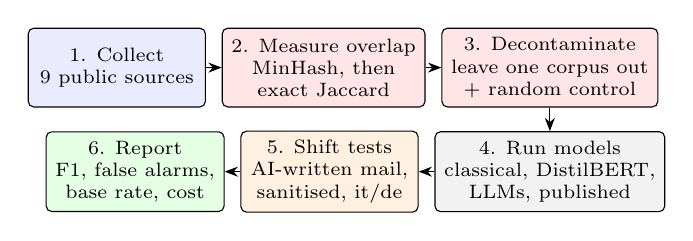
\begin{tikzpicture}[
  box/.style={draw, rounded corners=2pt, align=center, font=\scriptsize,
              minimum width=2.25cm, minimum height=1.0cm, fill=#1},
  box/.default=white, >=Stealth, node distance=0.3cm and 0.2cm]
\node[box=blue!8] (a) {1. Collect\\9 public sources};
\node[box=red!10, right=of a] (b) {2. Measure overlap\\MinHash, then\\exact Jaccard};
\node[box=red!10, right=of b] (c) {3. Decontaminate\\leave one corpus out\\+ random control};
\node[box=gray!10, below=of c] (d) {4. Run models\\classical, DistilBERT,\\LLMs, published};
\node[box=orange!12, left=of d] (e) {5. Shift tests\\AI-written mail,\\sanitised, it/de};
\node[box=green!10, left=of e] (f) {6. Report\\F1, false alarms,\\base rate, cost};
\draw[->] (a) -- (b); \draw[->] (b) -- (c); \draw[->] (c) -- (d); \draw[->] (d) -- (e); \draw[->] (e) -- (f);
\end{tikzpicture}
\caption{The pipeline. Steps 2 and 3, and the operating-point part of step 6,
are what earlier cross-corpus work does not do.}
\label{fig:pipeline}
\end{figure}

\section{Method}

Fig.~\ref{fig:pipeline} shows the pipeline. It has six steps, one script each.

\subsection{Overlap between corpora}

We compare every pair of the nine sources on the full cleaned corpora, before
sampling, at three levels.
\begin{itemize}
\item \textit{Exact raw}: MD5 of the text exactly as the model reads it.
\item \textit{Exact normalized}: MD5 of the body after lowercasing and
removing all whitespace. This is the check we used in our preliminary work.
\item \textit{Near duplicate}: MinHash~\cite{broder} with 128 permutations over
9-character shingles of the first 2{,}000 letters and digits of the body, with
locality sensitive hashing to find candidates. Two emails count as the same
if their estimated Jaccard similarity is at least 0.8.
\end{itemize}
We first tried 5-word shingles. They missed many copies, because the Kaggle
aggregate often deletes line breaks and glues two words together
(``cream?Isn't''). Character shingles over letters and digits ignore that. To
check the matcher, we took 400 random SpamAssassin emails that had no
normalized exact match in Kaggle and searched Kaggle by brute force. 59\% had a
Kaggle email with a true Jaccard of at least 0.8, the same rate MinHash
reported for that group, and manual reading confirmed they were the same
messages with different line breaks or a cut first word.

\subsection{Leave-one-corpus-out with decontamination}

For each of the six corpora $T$ we train on the other five and test on all of
$T$. We run this twice. In the \textit{raw} setting the training data is used
as it is. In the \textit{clean} setting we first remove every training email
that has a near duplicate in $T$. The difference in F1 between the two is the
inflation caused by leaked emails. The three test-only sets are scored with a
model trained on all six corpora, again with near duplicates of the test set
removed. As a reference we also report the usual in-corpus score, an 80/20
stratified split inside each corpus.

\subsection{Models}

\textit{Classical.} TF-IDF over word unigrams and bigrams (50{,}000 features,
minimum document frequency 2) with Logistic Regression or multinomial Naive
Bayes, as in our preliminary work.

\textit{DistilBERT.} \texttt{distilbert-base-uncased}~\cite{distilbert} fine-tuned
for one epoch, 128 tokens, batch 16, learning rate $5\times10^{-5}$, on a
stratified sample of 1{,}000 emails per training corpus (about 5{,}000 per
fold). It runs on the laptop CPU (Apple M1). Only the clean setting is run.

\textit{Small open LLMs.} Llama-3.2-1B, Llama-3.2-3B, Llama-3.1-8B,
Qwen-2.5-7B, Gemma-3-12B and Phi-4 (14B), all instruction-tuned and called
through OpenRouter. The system prompt asks whether the email is ``malicious or
unwanted (phishing, scam or spam) or legitimate'' and to answer with one word.
Temperature is 0, output is limited to 5 tokens, and emails are cut to 1{,}500
characters. An answer containing ``phish'', ``spam'' or ``malicious'' counts as
positive, one containing ``legit'' as negative. Anything else (for example a
refusal) counts as negative and is reported. An LLM never sees our training
data, so every test set is unseen for it. In the few-shot setting the prompt
holds four short examples (two positive, two negative) drawn from corpora
other than the test corpus, which keeps the leave-one-corpus-out rule.

\subsection{Metrics and cost}

We report F1 for the positive class, because accuracy hides the failure we care
about (a model that calls everything legitimate still gets high accuracy on a
mostly legitimate corpus). The headline robustness number is the mean F1 over
the six held-out corpora, with a 95\% interval from 1{,}000 bootstrap
resamples of the emails in each test set, plus the worst of the six. For
LLMs, cost is the sum of the \texttt{usage.cost} field that OpenRouter returns
for every call, divided by the number of emails. Local models have no API
cost. We report their inference time instead.

\section{Results}

\subsection{The corpora overlap far more than exact matching shows}

Table~\ref{tab:overlap} and Fig.~\ref{fig:overlap} show the overlap. Compared
exactly as a model reads them, SpamAssassin and Kaggle share only 2 emails.
With whitespace removed they share 3{,}850, and with near-duplicate matching
5{,}009, which is 86\% of SpamAssassin. The Kaggle set also contains 90\% of
Ling-Spam and 35\% of Enron, and more than half of Kaggle has a copy in Enron.
In other words, the Kaggle ``dataset'' is mostly three older corpora put
together, with formatting changed on the way. Anyone who deduplicates the usual
way, by exact text, would call these corpora independent. The older corpora
also overlap each other: 14\% of SpamAssassin has a near copy in Enron.

CEAS-08, TREC-07, Nazario and E-PhishLLM share almost nothing with any other
source. This gives us a natural control group for the next experiment.

\begin{figure}[t]
\centering
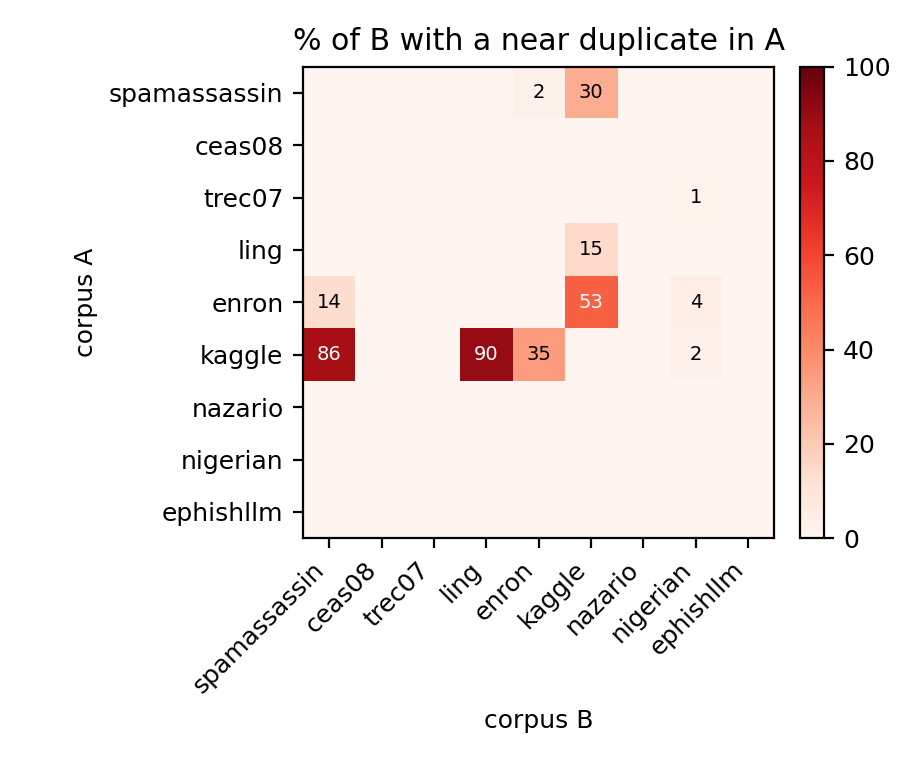
\includegraphics[width=0.88\columnwidth]{overlap_heatmap.png}
\caption{Near-duplicate overlap. Cell $(A,B)$ is the share of corpus $B$ that
has a near duplicate in corpus $A$.}
\label{fig:overlap}
\end{figure}

\begin{table}[t]
\caption{Emails of one corpus found inside another, at three levels of matching. Percentages are of the first corpus.}
\label{tab:overlap}
\centering\footnotesize
\setlength{\tabcolsep}{3pt}
\begin{tabular}{lrrr}
\toprule
Pair & Exact raw & No whitespace & Near duplicate \\
\midrule
SpamAssassin in Kaggle & 2 ($<$0.1\%) & 3,850 (66.3\%) & 5,009 (86.3\%) \\
Ling-Spam in Kaggle & 61 (2.1\%) & 62 (2.2\%) & 2,577 (90.2\%) \\
Enron in Kaggle & 3 ($<$0.1\%) & 187 (0.6\%) & 10,229 (34.5\%) \\
Kaggle in Enron & 3 ($<$0.1\%) & 188 (1.1\%) & 9,212 (52.6\%) \\
SpamAssassin in Enron & 0 (0.0\%) & 122 (2.1\%) & 793 (13.7\%) \\
Nigerian in TREC-07 & 2 ($<$0.1\%) & 2 ($<$0.1\%) & 42 (1.3\%) \\
\bottomrule
\end{tabular}
\end{table}


\subsection{Leaked emails inflate cross-corpus scores}

Table~\ref{tab:pairwise} repeats the one-corpus-to-one-corpus test from our
preliminary work. The Kaggle to SpamAssassin transfer, which looked almost
perfect (F1 0.966), falls to 0.666 once the 2{,}935 Kaggle training emails that
also appear in SpamAssassin are removed. Kaggle to Enron falls from 0.969 to
0.738. The ``good transfer'' was the model recognising emails it had already
seen.

Table~\ref{tab:inflation} shows the same effect in the leave-one-corpus-out
setting. Removing leaked emails lowers Logistic Regression F1 by 11.5 points
on Ling-Spam, 10.0 on SpamAssassin, 5.4 on Enron and 4.8 on Kaggle. For CEAS-08
and TREC-07, which share almost nothing with the other corpora, the change is
0.1 points or less. The inflation appears exactly where the overlap is, which
is strong evidence that leakage, and not some other difference between the
settings, causes it.

Fig.~\ref{fig:incorpus} puts the three settings side by side. The usual
in-corpus split gives 0.93 to 0.99. Honest leave-one-corpus-out testing gives
0.83 to 0.93. The in-corpus number overstates what the model will do on mail
from a new source by 4 to 15 points.

\begin{table}[t]
\caption{Single-corpus transfer with TF-IDF and logistic regression, before and after removing training emails that also appear in the test corpus. The last row is a pair that shares almost nothing.}
\label{tab:pairwise}
\centering\footnotesize
\setlength{\tabcolsep}{3pt}
\begin{tabular}{lrrr}
\toprule
Train $\rightarrow$ test & Removed & Raw F1 & Clean F1 \\
\midrule
Kaggle $\rightarrow$ SpamAssassin & 2,954 & 0.966 & 0.672 \\
Kaggle $\rightarrow$ Enron & 5,511 & 0.969 & 0.661 \\
Kaggle $\rightarrow$ Ling-Spam & 1,450 & 0.979 & 0.837 \\
SpamAssassin $\rightarrow$ Kaggle & 5,032 & 0.766 & 0.590 \\
SpamAssassin $\rightarrow$ Enron & 855 & 0.673 & 0.440 \\
CEAS-08 $\rightarrow$ TREC-07 & 6 & 0.737 & 0.734 \\
\bottomrule
\end{tabular}
\end{table}

\begin{table}[t]
\caption{Leave-one-corpus-out F1 of TF-IDF + Logistic Regression on the full held-out corpus. ``Removed'' is the number of training emails with a near duplicate in the test corpus. $\Delta$ is raw minus clean, in F1 points, for LogReg and Naive Bayes.}
\label{tab:inflation}
\centering\footnotesize
\setlength{\tabcolsep}{3pt}
\begin{tabular}{lrrrrrr}
\toprule
Held out & Removed & In-corpus & Raw & Clean & $\Delta$ LR & $\Delta$ NB \\
\midrule
SpamAssassin & 3,165 & 0.966 & 0.947 & 0.847 & +10.0 & +5.3 \\
Ling-Spam & 1,444 & 0.930 & 0.962 & 0.847 & +11.5 & +4.5 \\
Enron & 6,091 & 0.981 & 0.972 & 0.919 & +5.4 & +5.4 \\
Kaggle & 11,018 & 0.965 & 0.976 & 0.928 & +4.8 & +2.1 \\
CEAS-08 & 13 & 0.986 & 0.833 & 0.832 & +0.1 & +0.0 \\
TREC-07 & 7 & 0.985 & 0.871 & 0.871 & +0.0 & +0.1 \\
\bottomrule
\end{tabular}
\end{table}


\begin{figure}[t]
\centering
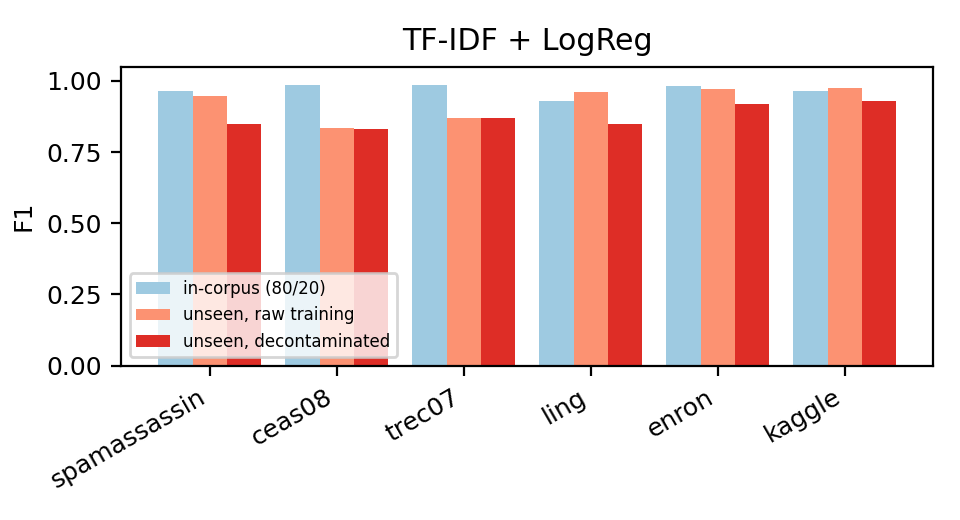
\includegraphics[width=0.95\columnwidth]{incorpus_vs_unseen.png}
\caption{TF-IDF + LogReg F1 per held-out corpus: in-corpus split, unseen
corpus with raw training data, and unseen corpus after decontamination.}
\label{fig:incorpus}
\end{figure}

\subsection{Comparing all models on unseen mail}

Table~\ref{tab:main} is the table our proposal promised: every model on the
same held-out emails, with robustness, AI phishing and cost in one place.
Fig.~\ref{fig:percorpus} breaks the scores down per test set.

\begin{table*}[t]
\caption{Main results. All numbers are on the same fixed evaluation emails. Trained models use decontaminated leave-one-corpus-out data. ``Unseen'' is the mean F1 over the six held-out corpora with a 95\% bootstrap interval, ``Worst'' the lowest of the six. FA is the false alarm rate, the share of legitimate emails flagged as phishing, averaged over the six corpora. AI phishing is F1 on E-PhishLLM. Nazario and Nigerian contain only positives, so we report recall. Cost is the measured OpenRouter charge in USD per 1{,}000 emails.}
\label{tab:main}
\centering\footnotesize
\setlength{\tabcolsep}{4.5pt}
\begin{tabular}{lrrrrrrrrr}
\toprule
Model & In-corpus & Unseen & 95\% CI & Worst & FA (\%) & AI phishing & Nazario rec. & Nigerian rec. & USD/1k \\
\midrule
Qwen-2.5-7B few-shot & -- & 0.937 & 0.925--0.948 & 0.844 & 4.8 & 0.598 & 0.847 & 1.000 & 0.074 \\
Qwen-2.5-7B & -- & 0.928 & 0.915--0.940 & 0.850 & 3.0 & 0.819 & 0.940 & 1.000 & 0.031 \\
TF-IDF + LogReg & 0.969 & 0.901 & 0.886--0.916 & 0.807 & 9.3 & 0.640 & 0.713 & 1.000 & local \\
Llama-3.2-3B few-shot & -- & 0.901 & 0.885--0.915 & 0.848 & 2.7 & 0.438 & 0.680 & 0.993 & 0.037 \\
TF-IDF + NB & 0.929 & 0.895 & 0.879--0.909 & 0.773 & 6.6 & 0.631 & 0.600 & 0.987 & local \\
DistilBERT & 0.975 & 0.891 & 0.875--0.906 & 0.838 & 6.3 & 0.493 & 0.760 & 0.947 & local \\
Gemma-3-12B & -- & 0.882 & 0.866--0.896 & 0.768 & 25.1 & 0.955 & 0.980 & 1.000 & 0.016 \\
Llama-3.1-8B & -- & 0.881 & 0.865--0.896 & 0.779 & 21.4 & 0.817 & 0.973 & 1.000 & 0.011 \\
Llama-3.2-3B & -- & 0.850 & 0.832--0.868 & 0.799 & 5.1 & 0.507 & 0.827 & 1.000 & 0.016 \\
Phi-4-14B & -- & 0.727 & 0.702--0.749 & 0.621 & 27.6 & 0.759 & 0.660 & 0.513 & 0.021 \\
Llama-3.2-1B & -- & 0.623 & 0.597--0.647 & 0.359 & 60.0 & 0.474 & 0.760 & 0.607 & 0.009 \\
\bottomrule
\end{tabular}
\end{table*}


\begin{figure}[t]
\centering
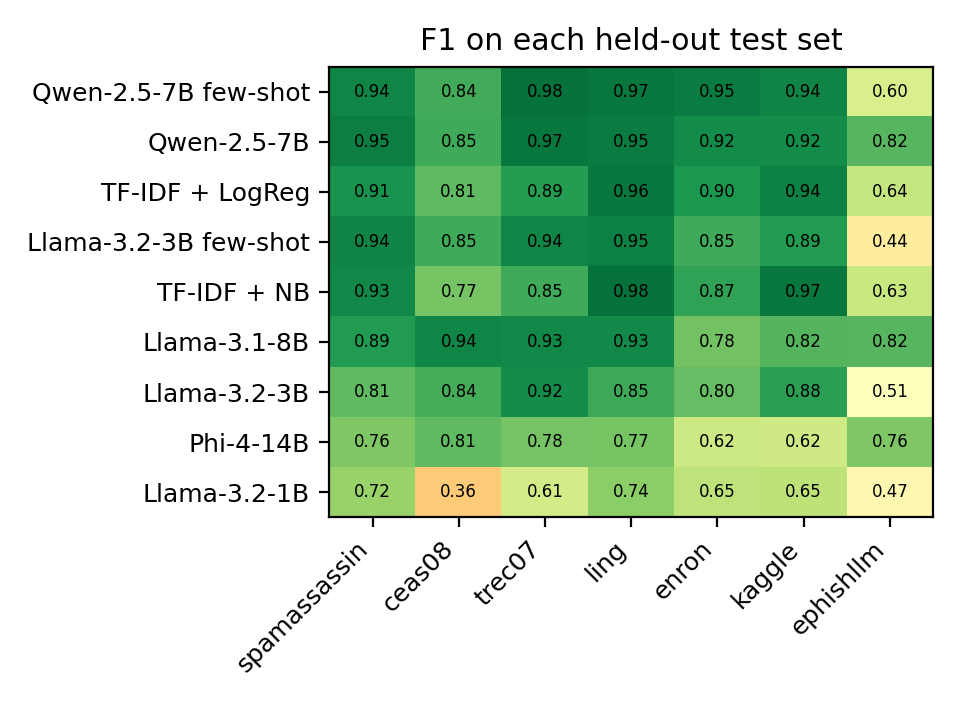
\includegraphics[width=\columnwidth]{per_corpus_f1.png}
\caption{F1 of every model on each held-out test set.}
\label{fig:percorpus}
\end{figure}

\textit{Small LLMs can match or beat trained models on unseen corpora.}
Zero-shot Qwen-2.5-7B reaches a mean F1 of 0.928 on the six held-out
corpora, above TF-IDF + LogReg (0.901) and although Qwen never
saw any of our training data.

\textit{AI-written phishing separates the models.} On E-PhishLLM the trained
models fall to 0.640 (LogReg) and 0.631 (Naive Bayes). They learned
what old spam looks like, and polished GPT-4o-mini phishing does not look like
old spam. Qwen-2.5-7B (0.819) and Llama-3.1-8B (0.817) hold up much better.

\textit{Few-shot examples help on old mail and hurt on new mail.} Four
examples drawn from the other corpora raise Qwen-2.5-7B from 0.928 to
0.937 on the held-out corpora, and Llama-3.2-3B from 0.850 to
0.901. The same examples lower AI-phishing F1 from 0.819 to 0.598
for Qwen and from 0.507 to 0.438 for Llama. The examples come from old
corpora, and they seem to anchor the model to what phishing looked like in
2002 to 2008. Few-shot also more than doubles the cost, because the prompt is
longer.

\textit{Bigger is not automatically better.} Phi-4 (14B) has a lower mean F1
(0.727) than the 3B and 8B Llama models. In 37\% of emails it ignored the
instruction to answer in one word and started an explanation (``As a large
language model\ldots'', ``Based on the content\ldots''), so no verdict fit in the
output.  Llama-3.2-1B is too weak for the task (0.623, with a
worst-corpus F1 of 0.359).

\subsection{Cost}

The measured cost of zero-shot classification ranges from 0.009 to
0.031 US dollars per 1{,}000 emails (Fig.~\ref{fig:cost}). Qwen-2.5-7B
costs 0.031 dollars per 1{,}000 emails, so screening 100{,}000 emails a month
would cost about 3.07 dollars. TF-IDF needs about 0.25 CPU seconds per
1{,}000 emails and no API. DistilBERT needs 0 minutes of laptop GPU time
per training fold and 0 seconds per 1{,}000 emails. The whole study,
18{,}000 LLM calls including discarded trials, cost 0.50 US dollars.

\begin{figure}[t]
\centering
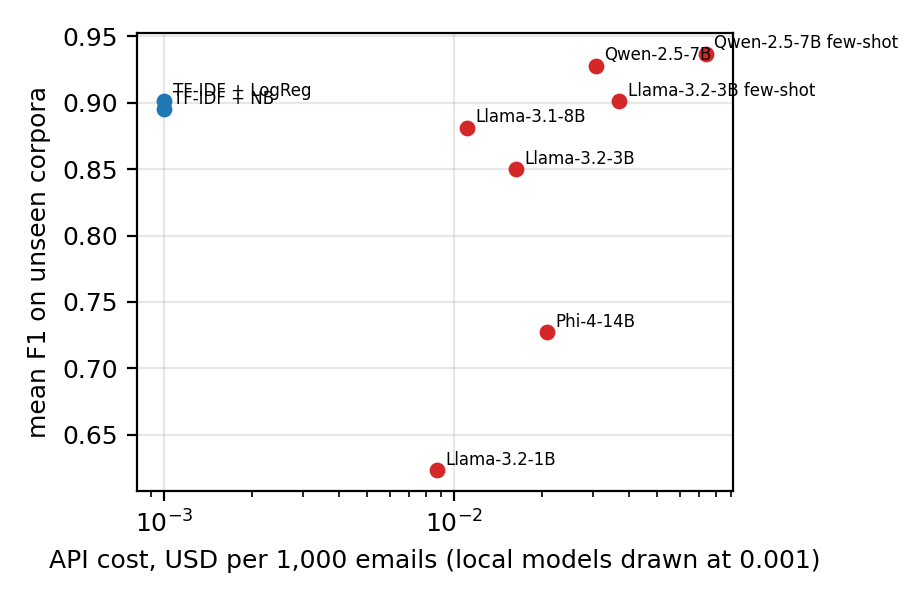
\includegraphics[width=\columnwidth]{f1_vs_cost.png}
\caption{Mean F1 on unseen corpora against measured API cost. Local models
have no API cost and are drawn at 0.001.}
\label{fig:cost}
\end{figure}

\section{Discussion}

\textit{Measure overlap before claiming generalization.} The clearest finding
here is about the benchmarks rather than the models. A paper that trains on the
Kaggle aggregate and tests on SpamAssassin is testing mostly on its own
training data, and exact-match deduplication does not reveal it because the
aggregate changed the line breaks. A near-duplicate pass over 170{,}000 emails
took five minutes on a laptop in our run, so there is no practical reason to
skip it before a cross-dataset claim. Our random-removal control also shows
that the effect is leakage and not the smaller training set, which is the first
question a careful reader asks.

\textit{In-corpus scores answer a different question.} The 97 to 99\% in the
literature is real, but it says how well a model recognises more mail from the
same collection. A mail server does not receive mail from the training
collection. On unseen corpora the same model loses several points; on
AI-written mail it loses many more; and the model with the best in-corpus score
in our table is among the weakest on AI-written phishing.

\textit{Know what the positive class is.} Only a fifth of the positive emails
in these corpora are phishing. Work that reports "phishing detection" on them
is largely reporting spam detection. This does not invalidate the corpora, but
a paper should either say which it means or, as we did, measure the split.

\textit{Choose an operating point, not a leaderboard position.} At the balanced
prevalence used in benchmarks, several models look similar. At a realistic
phishing rate the false alarm rate dominates, and models that share an F1
differ by an order of magnitude in how much legitimate mail they would flag.
The two-stage detectors show a more practical way to use a cheap model: a free
classical filter in front of an LLM cuts both the cost and the false alarms,
and the reverse order is the right shape for a quarantine queue that a person
reviews. Conformal deferral~\cite{triage} is the natural next step.

\textit{What we would deploy.} For an organisation with no GPU and a small
budget, a TF-IDF filter in front of zero-shot Qwen-2.5-7B is the best
combination we measured: it is the cheapest configuration in our tables and has
the lowest false alarm rate. If the budget allows a commercial API,
Gemini-3.1-Flash-Lite was better than every open model on every axis we
measured, which is an honest result even though it is not the one we hoped for.
Gemma-3-12B should be used only where a person reviews the output.

\textit{Test the shortcut you suspect, on the same emails.} The AI-written
corpus writes links as a placeholder that appears almost only in phishing mail,
and the obvious comparison, splitting the phishing emails by whether they carry
it, says the token is worth a large amount of recall. That comparison is
confounded, because the two halves are different kinds of attack. Removing the
token from the same emails moves the verdicts by almost nothing. We report both
because the quick test pointed the wrong way, and a reader who only ran it
would have drawn the opposite conclusion about this corpus.

\section{Limitations}

\begin{itemize}
\item \textit{Labels.} Four corpora count ordinary spam as positive. We measure
the split with an LLM annotator and a second annotator for agreement, but the
underlying labels stay as published, and the annotator is itself a model.
\item \textit{Sample size.} Each test set has 300 emails, 150 for the one-class
sets. The bootstrap interval on the mean F1 is about $\pm$0.015; the
leave-one-corpus-out jackknife is wider and is the number to read when asking
about a new corpus.
\item \textit{Input budgets differ by model family.} TF-IDF sees 20{,}000
characters, the LLMs 1{,}500, DistilBERT 128 word pieces. DistilBERT is
therefore the most truncated model and its row should be read as a lower bound.
\item \textit{Training budgets differ.} DistilBERT trains on about 5{,}000
emails per fold against 40{,}000 for the classical models, to fit the laptop.
\item \textit{LLM pre-training.} The legacy corpora may be inside the LLMs'
pre-training data~\cite{contamsurvey}. E-PhishLLM was released in 2025, after
most of these models, which makes it the most trustworthy of our tests, and the
published detectors we ran are contaminated by construction.
\item \textit{Providers.} OpenRouter routes each model to a provider of its
choosing, so a small part of the cost and a small part of the behaviour is
routing rather than the model.
\item \textit{Scope.} Text only, one prompt per model, one run. Headers, URLs
and attachments are ignored, and the Kaggle corpus has no subject line at all,
which is an unmeasured difference between it and the others.
\item \textit{Phishsense-1B} is evaluated through an ungated third-party merge
and with our own prompt, because the original repository and its prompt
template are gated. Its numbers may understate the released model.
\end{itemize}

\section{Conclusion}

Public phishing corpora overlap heavily, and in a way that exact matching
cannot see: most of the Kaggle aggregate has a near duplicate in another public
corpus. Removing those duplicates lowers cross-corpus F1 by up to 30 points for
a single pair, while removing the same number of emails at random changes
nothing. On decontaminated, unseen data a small open LLM used zero-shot is as
good as a trained classical model and much better on AI-written phishing, for a
few cents per thousand emails, though a current commercial model is still
ahead of all of them. Which model is best depends on the operating point: at a
realistic phishing rate the false alarm rate decides, and a free classical
filter in front of a small LLM beats either part alone on both cost and false
alarms. Finally, the corpora themselves deserve more scepticism than they
usually get: four fifths of their positive emails are spam rather than
phishing, and a corpus feature that looks like a shortcut needs a paired test
before it is believed, in either direction.
High accuracy on one dataset is easy. Honest evaluation is the hard part. All
code, raw model answers and results are public so that others can check and
extend this work.

\section*{Acknowledgment}
We thank our Computer Security course instructor at United International
University for the feedback on our literature review and proposal.


\begin{thebibliography}{99}

\bibitem{heiding}
F.~Heiding, B.~Schneier, A.~Vishwanath, J.~Bernstein, and P.~S. Park, ``Devising and detecting phishing emails using large language models,'' \emph{IEEE Access}, vol.~12, pp. 42131--42146, 2024.

\bibitem{koide}
T.~Koide, N.~Fukushi, H.~Nakano, and D.~Chiba, ``ChatSpamDetector: Leveraging large language models for effective phishing email detection,'' arXiv:2402.18093, 2024.

\bibitem{uddin}
M.~A. Uddin, M.~Mahiuddin, and I.~H. Sarker, ``An explainable transformer-based model for phishing email detection: A large language model approach,'' arXiv:2402.13871, 2024.

\bibitem{lin}
Z.~Lin, Z.~Liu, and H.~Fan, ``Improving phishing email detection performance of small large language models,'' arXiv:2505.00034, 2025.

\bibitem{kuikel}
S.~Kuikel, A.~Piplai, and P.~Aggarwal, ``Evaluating large language models for phishing detection, self-consistency, faithfulness, and explainability,'' arXiv:2506.13746, 2025.

\bibitem{alhuzali}
A.~Alhuzali, A.~Alloqmani, M.~Aljabri, and F.~Alharbi, ``In-depth analysis of phishing email detection: Evaluating the performance of machine learning and deep learning models across multiple datasets,'' \emph{Applied Sciences}, vol.~15, no.~6, 2025.

\bibitem{multiphish}
Y.~Xue, E.~Spero, M.~W. Woo, W.~Gao, and G.~Russello, ``MultiPhishGuard: An explainable and adaptive multi-agent LLM system for phishing email detection,'' arXiv:2505.23803, 2025.

\bibitem{phishsense}
S.~E. Blake, ``Phishsense-1B: A technical perspective on an AI-powered phishing detection model,'' arXiv:2503.10944, 2025.

\bibitem{ephishgen}
L.~Pajola, E.~Caripoti, S.~Banzer, S.~Pizzi, M.~Conti, and G.~Apruzzese, ``E-PhishGen: Unlocking novel research in phishing email detection,'' in \emph{Proc. ACM Workshop on Artificial Intelligence and Security (AISec)}, 2025.

\bibitem{champa}
A.~I. Champa, M.~F. Rabbi, and M.~F. Zibran, ``Curated datasets and feature analysis for phishing email detection with machine learning,'' in \emph{Proc. IEEE 3rd Int. Conf. Computing and Machine Intelligence (ICMI)}, 2024, pp. 1--7.

\bibitem{arp}
D.~Arp, E.~Quiring, F.~Pendlebury, A.~Warnecke, F.~Pierazzi, C.~Wressnegger, L.~Cavallaro, and K.~Rieck, ``Dos and don'ts of machine learning in computer security,'' in \emph{Proc. USENIX Security Symposium}, 2022, pp. 3971--3988.

\bibitem{kapoor}
S.~Kapoor and A.~Narayanan, ``Leakage and the reproducibility crisis in machine-learning-based science,'' \emph{Patterns}, vol.~4, no.~9, 2023.

\bibitem{broder}
A.~Z. Broder, ``On the resemblance and containment of documents,'' in \emph{Proc. Compression and Complexity of Sequences}, 1997, pp. 21--29.

\bibitem{distilbert}
V.~Sanh, L.~Debut, J.~Chaumond, and T.~Wolf, ``DistilBERT, a distilled version of BERT: smaller, faster, cheaper and lighter,'' arXiv:1910.01108, 2019.

\end{thebibliography}


\end{document}
